\chapter{Aspectos Teóricos}

% TODO: escribir la idea general

\noindent
En este capítulo cimentamos las bases teóricas necesarias para resolver instancias particulares de
programas lineales enteros. En primer lugar, la sección de Prerrequisitos recopila resultados
básicos de teoría de números y de programación lineal para refrescar la memoria del lector. En
segundo lugar, la sección de Fundamentos comienza con definiciones y enunciados obtenidos de
\cite{herr}, los cuales utilizaremos para obtener resultados que, en pleno conocimiento del autor,
son originales. El problema fundamental que permitirá construir incrementalmente nuestro algoritmo
es
\begin{subequations}
	\label{theory:formulation}
	\begin{align}
		\max_{\vec{x} \in \Z^n} \quad
			& \vec{p}^T\vec{x}, \label{theory:objective} \\
		\text{s.a.} \quad
			& \vec{p}^T\vec{x} \leq u, \label{theory:constraint:budget} \\
			& \vec{x} \geq \vec{0}. \nonumber
	\end{align}
\end{subequations}

Por ello mismo, es razonable suponer que $\vec{p}_i \neq 0$ para cualquier $i \in \lbrace 1, \ldots,
n \rbrace$. En la sección de Fundamentos analizaremos a profundidad este problema, cuyo punto de
culminación será el Teorema \ref{theory:th:feasibility}. Veremos que es recomendable separar en dos
partes el análisis de este problema: el caso $p_i < 0$ para alguna $i \in \lbrace 1, \ldots, n
\rbrace$; y el caso $\vec{p} \geq \vec{0}$. Los siguientes dos capítulos examinarán respectivamente
estos casos. Por el momento, cabe destacar que el segundo caso será de mayor interés y tendrá mayor
aplicabilidad en problemas reales, pues es una instancia particular del Problema de la Mochila. No
obstante, el caso $\vec{p}_i < 0$ también será de utilidad para exhibir casos particulares en donde
el algoritmo de Ramificación y Acotamiento obtiene un rendimiento deficiente.

\section{Prerrequisitos}
\noindent
En los siguientes capítulos usaremos extensivamente resultados básicos de teoría de números y de
programación lineal, por lo que es provechoso recopilarlos en esta primera sección. En
particular, destaca la importancia de las ecuaciones lineales diofantinas para la construcción
de nuestro algoritmo. En esta sección el autor consideró pertinente no incluir demostraciones, pues los
enunciados son mostrados en cualquier clase de álgebra superior, programación lineal, o
investigación de operaciones, por ejemplo. La referencia principal para la parte de teoría de
números es \cite{carmen}, mientras que la de programación lineal es \cite{alex}.

\subsection{Teoría de Números}
\subsubsection{Máximo común divisor y mínimo común múltiplo}
\noindent
En primer lugar, introducimos el símbolo de relación ``$\mid$'' para indicar divisibilidad. Dados
dos enteros $a, b$, decimos que $b$ divide a $a$ (y escribimos $b \mid a$) si y solo si existe un
entero $k$ tal que $a = k \cdot b$. Así también, denotamos el conjunto de divisores de $a$ como
\begin{equation*}
	D(a) \coloneq \lbrace b \in \Z \vcentcolon b \mid a \rbrace.
\end{equation*}
Si $a$ es distinto de cero, encontramos que $D(a)$ es finito, puesto que si $b \mid a$, entonces
$|b| \leq |a|$, lo cual implica que $|D(a)| \leq 2|a|$. En caso de que $a$ sea nulo, obtenemos $D(a)
= \Z$. Observemos también que $\lbrace -1, 1 \rbrace \subseteq D(a)$ para todo entero $a$.

\begin{definition}
	\label{prerreq:def:gcd}
	Sean $a_1, \ldots, a_n$ enteros no todos iguales a cero, entonces definimos su máximo común
	divisor $d$ como el elemento maximal del conjunto $\bigcap_{i=1}^{n}D(a_i)$, y escribimos $d =
	\gcd{a_1, \ldots, a_n}$. Si $d = 1$, entonces decimos que $a_1, \ldots, a_n$ son coprimos.
\end{definition}

Puesto que $a_i \neq 0$ para alguna $i$ en la definición anterior, encontramos que el conjunto
$\bigcap_{i=1}^{n}D(a_i)$ es finito y, como también es no vacío, en efecto existe un elemento maximal.
Es decir, el máximo común divisor $d$ siempre está bien definido.

% FIX: no me gusta la redacción
\begin{observation}
	No porque una colección de enteros sea coprima ($\gcd{a_1, \ldots, a_n} = 1$) se sigue que
	estos enteros sean coprimos a pares ($\gcd{a_i, a_j} = 1$ para todo $i, j$). Por ejemplo,
	los enteros 1, 3 y 3 son coprimos pero evidentemente 3 y 3 no lo son.
\end{observation}

\begin{definition}
	Decimos que $c \in \Z$ es una combinación lineal entera de un conjunto de enteros $a_1, \ldots,
	a_n$ si existen enteros $x_1, \ldots, x_n$ tales que $c = a_1x_1 + \cdots + a_nx_n$.
\end{definition}

El siguiente teorema, a pesar de su simpleza, es central para los resultados obtenidos en esta
tesis.
\begin{theorem}
	\label{prerreq:th:bezout}
	Sea $d$ un entero y sean $a_1, \ldots, a_n$ una colección de enteros no todos iguales a cero.
	Entonces $d = \gcd{a_1, \ldots, a_n}$ si y solo si $d$ es la mínima combinación lineal entera
	positiva de $a_1, \ldots, a_n$.
\end{theorem}

% TODO: agregar un ejemplo

\begin{corollary}
	\label{prerreq:cor:gcd}
	Si $d = \gcd{a_1, \ldots, a_n}$, entonces $\gcd{\frac{a_1}{d}, \ldots, \frac{a_n}{d}} = 1$.
\end{corollary}

Además del máximo común divisor, requeriremos al mínimo común múltiplo, empero en menor medida. Sea
$a$ un entero y denotamos el conjunto de sus múltiplos como
\begin{equation*}
	M(a) \coloneq \lbrace x \in \Z \vcentcolon a \mid x \rbrace.
\end{equation*}
Si $a$ es nulo, entonces $M(a) = \lbrace 0 \rbrace$. En caso contrario encontramos que $M(a)$ es un
conjunto infinito. Ánalogamente a la Definición \ref{prerreq:def:gcd}, definimos el mínimo común
múltiplo $m$ de una colección de enteros $a_1, \ldots, a_n \in \Z \setminus \lbrace 0 \rbrace$ como
el elemento minimal de $\N \cap \bigcap_{i=1}^{n}M(a_i)$. Escribimos $m = \lcm{a_1, \ldots, a_n}$.
Para observar que está bien definido, basta mencionar que el producto $|a_1 \cdots a_n|$ es un
elemento de la intersección y por lo tanto esta es no vacía.

\subsubsection{Ecuaciones lineales diofantinas}

\noindent
Sea $c \in \Z$ y sean $a_1, \ldots, a_n$ enteros. Una ecuación lineal diofantina es una ecuación
donde queremos encontrar enteros $x_1, \ldots, x_n$ que satisfagan
\begin{equation*}
	a_1x_1 + \cdots + a_nx_n = c.
\end{equation*}
Será de nuestro interés en las siguientes secciones resolver iterativamente este tipo de ecuaciones.
Por el momento basta mencionar que podemos enfocarnos en el caso $n = 2$ sin ninguna pérdida de
generalidad. No obstante, los resultados se mantienen para cualquier $n \in \N$. Los siguientes
enunciados abordan el problema de determinar existencia y unicidad para las ecuaciones lineales
diofantinas, así como la construcción de sus soluciones.

\begin{theorem}[Existencia]
	\label{prerreq:th:existence}
	Sean $a, b \in \Z$, no ambos cero. La ecuación $ax + by = c$ tiene solución si y solo si
	$\gcd{a, b} \mid c$.
\end{theorem}

Para construir el conjunto de soluciones a una ecuación lineal diofantina, encontramos primero una
solución particular.
\begin{definition}
	\label{prerreq:def:bezout}
	Sea $d \coloneq \gcd{a, b}$ y sean $x', y'$ enteros tales que $ax' + by' = d$ (c.f.
	\ref{prerreq:th:bezout}). Decimos entonces que $x', y'$ son coeficientes de Bézout asociados a
	$a, b$, respectivamente.
\end{definition}

\begin{observation}
	Los coeficientes de Bézout asociados a un par de enteros no son únicos. En efecto, si $x', y'$
	son coeficientes de Bézout de $a, b$, entonces $x' + b$, $y' - a$ también lo son:
	\begin{equation*}
		a(x' + b) + b(y' - a) = ax' + by' + ab - ab = ax' + by' = d.
	\end{equation*}
	Para fines de esta tesis basta la existencia de estos coeficientes, por lo que decimos de manera
	indistinta ``los coeficientes de Bézout'' y ``una elección de coeficientes de Bézout''.
\end{observation}

Definamos $d \coloneq \gcd{a, b}$ y supongamos que la ecuación $ax + by = c$ tiene solución.
Entonces $d \mid c$, por lo que existe $c' \in \Z$ tal que $c = c' \cdot d$. Sean $x', y'$ los
coeficientes de Bézout asociados a $a, b$ respectivamente. Así,
\begin{equation*}
	a(c' \cdot x') + b(c' \cdot y') = c'(ax' + by') = c'd = c,
\end{equation*}
por lo que $(c' \cdot x', c' \cdot y')$ es una solución particular de la ecuación $ax + by = c$.

\begin{theorem}[Construcción]
	\label{prerreq:th:construction}
	Sea $(x_0, y_0)$ una solución particular de la ecuación lineal diofantina $ax + by = c$.
	Entonces todas las soluciones de la ecuación están dadas por
	\begin{equation}
		\label{prerreq:eq:construction}
		\begin{cases}
			x = x_0 + \frac{b}{d}t, \\
			y = y_0 - \frac{a}{d}t,
		\end{cases}
	\end{equation}
	donde $d \coloneq \gcd{a, b}$ y $t \in \Z$.
\end{theorem}

% TODO: agregar un ejemplo

\subsection{Programación lineal}


\section{Fundamentos}
\noindent
Esta sección constituye el primer paso para la construcción de nuestro algoritmo. Se divide en dos
partes. Primeramente damos a conocer las definiciones y enunciados provistos por \cite{herr}, al
mismo tiempo que hacemos un par de observaciones. Esta primera parte puede darse por concluida una
vez citado el Teorema \ref{phase-1:th:cover}. Así también, es importante aclarar que el autor
tradujo libremente algunos términos a falta de encontrar fuentes en español que hicieran uso de
ellos. A saber, el autor decidió nombrar ``vectores esencialmente enteros'' a los
\textit{projectively rational vectors} y ``capas enteras'' a los \textit{c-layers} en las
Definiciones \ref{theory:def:rational} y \ref{phase-1:def:c-layer}, respectivamente.

En la segunda parte de esta sección comenzamos con nuestro análisis del problema
(\ref{theory:formulation}). La razón de considerarlo fundamental para esta tesis fue mencionado en
el capítulo de Motivación, pero lo repetimos una vez más: en esta clase de problemas el vector es
ortogonal a la única restricción, y esto implica que el problema relajado tenga una infinidad de
soluciones. Hemos observado que, en presencia de este fenómeno, el algoritmo de Ramificación y
Acotamiento no divide la región factible de manera óptima. Por ello investigamos formas alternativas
para atacar este problema antes de hacer la separación de casos $\vec{p}_i < 0$ o $\vec{p} \geq
\vec{0}$.
\begin{definition}
	\label{theory:def:rational}
	Decimos que un vector $\vec{v} \in \R^n \setminus \lbrace 0 \rbrace$ es esencialmente
	entero si existe un vector $\vec{w} \in \Z^n$ y un escalar $k \in \R$ tal que $\vec{v} =
	k\vec{w}$. Además, decimos que $\vec{w}$ es el múltiplo coprimo de $\vec{v}$ si sus entradas son
	coprimas (c.f. Definición \ref{prerreq:def:gcd}) y si su primera entrada $\vec{v}_1$ es no
	negativa.
\end{definition}
En otras palabras, decimos que $\vec{v}$ es esencialmente entero si es un múltiplo real de un vector
entero.
\begin{example}
	El vector $\left(-\sqrt{2}, 1/\sqrt{2}\right)^T = \sqrt{2}(-1, 1/2)^T$ es esencialmente entero
	y $(2, -1)^T$ es su múltiplo coprimo. Contrariamente, el vector $(\sqrt{2}, \sqrt{3})^T$ no es
	esencialmente entero.
\end{example}
\begin{observation}
	Todo vector $\vec{v}$ cuyas entradas son racionales ($\vec{v} \in \Q^n$) es esencialmente
	entero. En efecto, $\vec{v}_i = \frac{p_i}{q_i}$ para algunos enteros $p_i$ y $q_i$ con $q_i$
	distinto de cero. Si definimos $q \coloneq \lcm{q_1, \ldots, q_n} \neq 0$ y $\vec{w} \coloneq
	q\vec{v}$, se sigue que $\vec{v} = \frac{1}{q}\vec{w}$ y también $\vec{w} \in \Z^n$.
\end{observation}
\begin{observation}
	Todo vector $\vec{v}$ esencialmente entero tiene a lo más dos vectores coprimos asociados. Sean
	$k \in \R$ y $\vec{w} \in \Z^n$ tales que $\vec{v} = k\vec{w}$. Entonces
	\begin{equation*}
		\pm \frac{1}{\gcd{\vec{w}_1, \ldots, \vec{w}_n}}\vec{w}
	\end{equation*}
	son dos vectores cuyas entradas son coprimas, de acuerdo al Corolario \ref{prerreq:cor:gcd}. Si
	$\vec{w}_1 = 0$, estos representan el mismo vector, y si $\vec{w}_1 \neq 0$ entonces solo uno de
	estos dos vectores es el múltiplo coprimo de $\vec{v}$. Independientemente del caso, el múltiplo
	coprimo de todo vector esencialmente entero es único.
\end{observation}

Porque todo número representable en cualquier sistema de aritmética finita es necesariamente
racional, decidimos enfocar nuestro análisis en vectores esencialmente enteros. Desde el punto de
vista puramente teórico, esta condición reduce drásticamente el tipo de programas lineales que
podemos resolver. No obstante, esta clase de vectores es un poco más general que los considerados en
otros textos de programación lineal, por ejemplo, \cite{martello} y \cite{alex} toman en cuenta
vectores puramente racionales. En \cite{herr} se revelan propiedades de los vectores esencialmente
enteros que reproducimos aquí y que nos permitirán plantear ecuaciones lineales diofantinas cuyas
soluciones otorgan candidatos para puntos óptimos de un problema lineal.

\begin{definition}
	\label{phase-1:def:c-layer}
	Sea $\vec{v} \in \R^n$ un vector esencialmente entero y sea $t \in \R$ un escalar. Decimos que
	su hiperplano afino asociado
	\begin{equation}
		\label{phase-1:def:affine-hyperplane}
		H_{\vec{v}, t} \coloneq \ker{\vec{x} \mapsto \vec{v}^T\vec{x}} + t\vec{v}
		= \lbrace \vec{v}^{\perp} + t\vec{v} \vcentcolon \vec{v}^T\vec{v}^{\perp} = 0 \rbrace
	\end{equation}
	es una capa entera si contiene al menos un punto entero.
\end{definition}
Observemos que todo hiperplano afino $H_{\vec{v}, t}$ es invariante ante reescalamientos en
$\vec{v}$. Es decir, si $r \in \R \setminus \lbrace 0 \rbrace$ es un escalar, entonces $H_{\vec{v},
t} = H_{r\vec{v}, t/r}$. En particular, el conjunto de hiperplanos afinos asociados a un vector
$\vec{v}$ esencialmente entero es igual al conjunto de hiperplanos afinos asociados a su múltiplo
coprimo $\vec{w}$. Ahora bien, cualquier vector coprimo induce una familia de capas enteras y,
sorprendentemente, esa familia forma una cobertura de $\Z^n$, como lo indica el Teorema
\ref{phase-1:th:cover}.

\begin{figure}
	\centering
	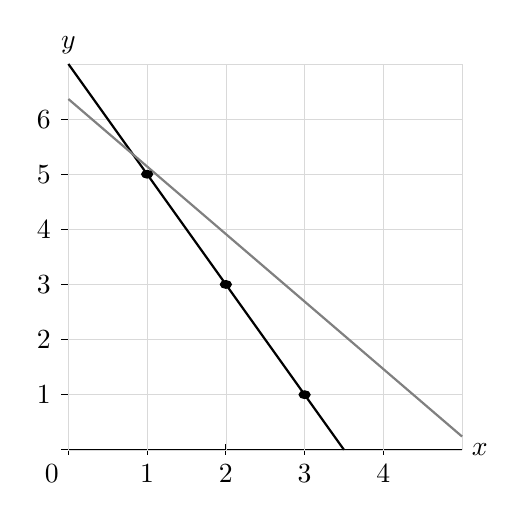
\begin{tikzpicture}[scale=1.0, xscale=1, yscale=0.7]
		\centering
		\draw (0,0) -- (5,0) node[right] {\(x\)};
		\draw (0,0) -- (0,7) node[above] {\(y\)};
		% Add tick marks (optional)

		\foreach \x in {1,2,3,4}
			\draw (\x,0.1) -- (\x,-0.1) node[below] {\x};

		\foreach \y in {1,2,3,4,5,6}
			\draw (0.1,\y) -- (-0.1,\y) node[left] {\y};

		\draw (0,0.1) -- (0, -0.1) node[below left] {0};
		\draw (0.1,0) -- (-0.1, 0) node[below left] {};

		\draw[very thin, gray!30] (0,0) grid (5,7);

		\draw[thick, black, domain=0:3.5] plot (\x, {7 - 2*\x}) node[right] {};
		\draw[thick, gray, domain=0:5.0] plot (\x, {9/sqrt(2) - sqrt(1.5)*\x}) node[right] {};

		\filldraw[black] (3,1) circle (2pt) node[below right] {};
		\filldraw[black] (2,3) circle (2pt) node[above right] {};
		\filldraw[black] (1,5) circle (2pt) node[above left] {};
	\end{tikzpicture}
	\caption{Representación de una capa entera (en negro) junto a un hiperplano afino que no es capa
	entera (en gris). La capa entera tiene como parámetros $\vec{v} = (2, 1)^T$ y $t = 1.4$,
	mientras que los del hiperplano afino son $\vec{v} = (\sqrt{3}, \sqrt{2})^T$ y $t = 1.4$.}
	\label{phase-1:fig:c-layer}
\end{figure}

\begin{lemma}
	\label{phase-1:lemma:layer}
	Sean $\vec{v}, \vec{x} \in \R^n$ con $\vec{v}$ distinto de cero. Entonces $\vec{x} \in
	H_{\vec{v}, t_{\vec{x}}}$, donde $t_{\vec{x}} \coloneq \frac{\vec{v}^T\vec{x}}{\norm{\vec{v}}^2}$.
\end{lemma}

\begin{theorem}
	\label{phase-1:th:cover}
	Sea $\vec{v} \in \R^n$ un vector esencialmente entero y sea $\vec{w}$ su múltiplo coprimo.
	Entonces la familia de capas enteras $\left\lbrace H_{\vec{w}, k\norm{\vec{w}}^{-2}} \vcentcolon k
			\in \Z \right\rbrace$ cubre a $\Z^n$.
\end{theorem}

Pasemos a considerar el programa lineal (\ref{theory:formulation}) donde $\vec{p}$ es un vector
esencialmente entero y $\vec{q}$ es su múltiplo coprimo. Supongamos que $\vec{p}_i \neq 0$ para todo
$i \in \lbrace 1, \ldots, n \rbrace$, por lo que también se cumple que $\vec{q}_i \neq 0$. Comúnmente
a la función objetivo (\ref{theory:objective}) le daremos el nombre de utilidad y a la restricción
(\ref{theory:constraint:budget}) la llamaremos restricción presupuestaria, así como presupuesto al
lado derecho de esta restricción.
\begin{observation}
	Debido a la restricción presupuestaria, encontramos que el politopo está acotado por arriba. Así
	pues, el problema o bien es infactible, o bien tiene una utilidad finita.
\end{observation}

Cada escalar $t \in \R$ induce un hiperplano afino $H_{\vec{p}, t}$ donde se cumple que todo punto
$\vec{x} \in H_{\vec{p}, t}$ tiene un mismo nivel de utilidad. Como observamos previamente,
\begin{equation*}
	\left \lbrace H_{\vec{p}, t} \vcentcolon t \in \R \right\rbrace
	=
	\left \lbrace H_{\vec{q}, t} \vcentcolon t \in \R \right\rbrace.
\end{equation*}
A causa del Teorema \ref{phase-1:th:cover}, somos capaces de caracterizar todos los puntos enteros a
partir de $\vec{q}$. Aún más, obtenemos una enumeración de las capas enteras que cubren $\Z^n$, lo
cual nos permite determinar si la $k$-ésima capa entera contiene puntos factibles para el problema.

El nivel de utilidad para la $k$-ésima capa entera es $k$. En efecto, si $\vec{x} \in H_{\vec{q},
k\norm{\vec{q}}^{-2}}$, tenemos
\begin{equation*}
	\vec{x} = \vec{q}^{\perp} + k\norm{\vec{q}}^{-2}\vec{q},
\end{equation*}
donde $\vec{q}^{\perp}$ es un vector ortogonal a $\vec{q}$. Por lo tanto,
\begin{equation*}
	\vec{q}^T\vec{x} = \vec{q}^T\vec{q}^{\perp} + k\norm{\vec{q}}^{-2}\vec{q}^T\vec{q}
	= 0 + k \norm{\vec{q}}^{-2} \norm{\vec{q}}^{2} = k.
\end{equation*}

Para respetar la restricción presupuestaria, podemos encontrar el entero $\eta$ más grande que
satisfaga $\vec{q}^T\vec{x} \leq u$ para todo $\vec{x} \in H_{\vec{q}, \eta\norm{\vec{q}}^{-2}}$.
Diremos que $\eta$ es el primer entero que satisface la restricción presupuestaria, o bien que
$H_{\vec{q}, \eta\norm{\vec{q}}^{-2}}$ es la primera capa entera que satisface el presupuesto. De
esta manera, encontramos que las capas enteras que satisfacen el presupuesto son parametrizadas por
$k \in \lbrace \eta, \eta - 1, \ldots \rbrace$. Debido a la observación anterior, se cumple
inmediatamente que $\vec{q}^T\vec{x} = k$. Deducimos que si la $\eta$-ésima capa entera contiene
puntos no negativos, entonces las soluciones se encuentran en esa capa. En caso contrario,
descendemos a la $(\eta - 1)$-ésima capa entera y buscamos puntos enteros no negativos, etcétera.
\begin{lemma}
	\label{phase-1:lemma:eta}
	Sea $\vec{p} \in \R^n$ un vector esencialmente entero y sea $\vec{q}$ su múltiplo coprimo, de
	manera que $\vec{p} = m\vec{q}$ para algún escalar $m \in \R \setminus \lbrace 0 \rbrace$.
	Entonces la primera capa entera $H_{\vec{q}, \eta \norm{\vec{q}}^{-2}}$ que satisface el
	presupuesto está parametrizada por $\eta \coloneq \lfloor u/m \rfloor$.
\end{lemma}
\begin{proof}
	Sea $\vec{x}$ tal que $\vec{p}^T\vec{x} \leq u$. Entonces buscamos el mayor entero $\eta$ que
	satisfaga $\vec{q}^T\vec{x} \leq u/m$ para todo $\vec{x} \in H_{\vec{q},
	\eta\norm{\vec{q}}^{-2}}$. Por el Lema \ref{phase-1:lemma:layer} sabemos que
	\begin{equation*}
		\eta\norm{\vec{q}}^{-2} = \frac{\vec{q}^T\vec{x}}{\norm{\vec{q}}^2} \leq
		\frac{u/m}{\norm{\vec{q}}^2},
	\end{equation*}
	de donde se sigue inmediatamente que $\eta = \lfloor u/m \rfloor$.
\end{proof}
\begin{theorem}
	\label{theory:th:feasibility}
	Sea $\vec{p} \in \R^n$ un vector esencialmente entero y sea $\vec{q}$ su múltiplo coprimo.
	Entonces se cumple lo siguiente con respecto al problema (\ref{theory:formulation}):
	\begin{enumerate}
		\item El problema es infactible si y solo si $\vec{q} > \vec{0}$ y $u < 0$.
		\item Si $\vec{q}_i < 0$ para algún $i \in \lbrace 2, \ldots, n
			\rbrace$, entonces la $\eta$-ésima capa entera contiene un número infinito de puntos
			factibles.
		\item Si el problema es factible y $\vec{q} > \vec{0}$, entonces la $k$-ésima capa entera
			contiene un número finito de puntos factibles, donde $k \in \lbrace \eta, \eta - 1,
			\ldots 0 \rbrace$.
	\end{enumerate}
\end{theorem}
\begin{proof} \hfill
	\begin{enumerate}
		\item Supongamos que $\vec{q} \geq 0$ y $u < 0$. Si $\vec{x} \in \Z_{\geq \vec{0}}^n$
			entonces $\vec{q}^T\vec{x} \geq 0 > u$ y por lo tanto $\vec{x}$ no es factible. Luego,
			\begin{equation*}
				\Z_{\geq \vec{0}}^{n} \cap \lbrace \vec{x} \vcentcolon \vec{q}^T\vec{x} 
				\leq u \rbrace = \emptyset,
			\end{equation*}
			y el problema no es factible. Mostramos la otra implicación por contraposición. Si $u
			\geq 0$ observamos que $\vec{0}$ es factible. Se debe cumplir $u < 0$. Similarmente, si
			$\vec{q}_i < 0$ para algún $i \in \lbrace 2, \ldots, n \rbrace$, encontramos que $\lceil
			u/\vec{q}_i \rceil\vec{e}_i \in \Z^n$ es factible:
			\begin{equation*}
				\vec{q}^T\left\lceil \frac{u}{\vec{q}_i} \right\rceil\vec{e}_i
				= \vec{q}_i \left\lceil \frac{u}{\vec{q}_i} \right\rceil
				\leq \vec{q}_i \frac{u}{\vec{q}_i} = u,
			\end{equation*}
			además, como $u < 0$, concluimos que $\lceil u/\vec{q}_i \rceil\vec{e}_i$ es no negativo.
		\item Como $\vec{q}$ es un vector cuyas entradas son coprimas, sabemos de una generalización
			del Teorema \ref{prerreq:th:existence} que existe $\vec{x} \in \Z^n$ tal que
			$\vec{q}^T\vec{x} = \eta$. Definamos los siguientes conjuntos de índices
			\begin{equation*}
				I^+ \coloneq \lbrace i \vcentcolon q_i > 0 \rbrace,
				\quad I^- \coloneq \lbrace i \vcentcolon q_i < 0 \rbrace.
			\end{equation*}
			Cabe resaltar que estos dos conjuntos forman una partición de $\lbrace 1, \ldots,
			n\rbrace$. Podemos escoger escalares positivos $c_1, \ldots, c_n$ que satisfagan
			simultáneamente
			\begin{align}
				x_j + \sum_{i \in I^+}\vec{q}_ic_i &\geq 0, \quad \forall j \in I^-,
				\label{theory:pf:1} \\
				x_i - \sum_{j \in I^-}\vec{q}_jc_i &\geq 0, \quad \forall i \in I^+.
				\label{theory:pf:2}
			\end{align}
			Definamos el vector $\vec{x}^+ \in \Z^n$ de manera que
			\begin{equation*}
				\vec{x}^+_k \coloneq \begin{cases}
					x_k + \sum_{i \in I^+}\vec{q}_ic_i, \quad k \in I^-, \\
					x_k - \sum_{j \in I^-}\vec{q}_jc_k, \quad k \in I^+.
				\end{cases}
			\end{equation*}
			Se verifica que $\vec{x}^+$ es no negativo y, además,
			\begin{align*}
				\vec{q}^T\vec{x}^+
				&= \vec{q}^T\vec{x}
				+ \sum_{k \in I^-}\sum_{i \in I^+}\vec{q}_k\vec{q}_ic_i
				- \sum_{k \in I^+}\sum_{j \in I^-}\vec{q}_k\vec{q}_jc_k \\
				&= \eta
				+ \sum_{j \in I^-}\sum_{i \in I^+}\vec{q}_j\vec{q}_ic_i
				- \sum_{i \in I^+}\sum_{j \in I^-}\vec{q}_i\vec{q}_jc_i \\
				&= \eta.
			\end{align*}
			Así pues, tenemos existencia. Para concluir que hay un número infinito de puntos, basta
			observar que si la elección de coeficientes $c_1, \ldots, c_n$ satisface ambas
			desigualdades (\ref{theory:pf:1}) y (\ref{theory:pf:2}), entonces cualquier múltiplo
			positivo de estos coeficientes también las satisface.
		\item Se sigue que $u \geq 0$. Definamos
			\begin{equation}
				\label{theory:pf:p_k}
				P_k \coloneq H_{\vec{q}, k\norm{\vec{q}}^{-2}} \cap \Z_{\geq \vec{0}}^n
				= \left\lbrace \vec{x} \in \Z^n \vcentcolon \vec{q}^T\vec{x} = k,
					\vec{x} \geq \vec{0} \right\rbrace.
			\end{equation}
			Observemos que $P_k = \emptyset$ para todo $k$ negativo, pues $\vec{q} > \vec{0}$ y por
			lo tanto $\vec{q}^T\vec{x} \geq 0$ para cualquier $\vec{x}$ no negativo. Esto implica que
			ningún punto sobre capas enteras con parámetros negativos es factible.

			Sea $k \in \lbrace \eta, \eta - 1, \ldots, 0 \rbrace$. La capa entera $H_{\vec{q},
			k\norm{\vec{q}}^{-2}}$ interseca los ejes positivos en $\frac{k}{\vec{q}_i}\vec{e}_i$.
			Definamos $\ell_i \coloneq \lceil k/\vec{q}_i \rceil$. No es difícil ver que
			$H_{\vec{q}, k\norm{\vec{q}}^{-2}}$ está contenido en el prisma cuyas aristas son $[0,
			\ell_i]$ y, por lo tanto,
			\begin{equation*}
				P_k \subseteq \prod_{i = 1}^{n} [0, \ell_i] \cap \Z^n = \prod_{i = 1}^{n}
				\left( [0, \ell_i] \cap \Z \right).
			\end{equation*}
			Pero $\left| [0, \ell_i] \cap \Z \right| = \ell_i + 1$. Así,
			\begin{equation*}
				|P_k| \leq \prod_{i = 1}^{n} (\ell_i + 1) < \infty.
			\end{equation*}
			Entonces la $k$-ésima capa entera contiene un número finito de puntos factibles.
	\end{enumerate}
\end{proof}
% TODO: hay una expresión bonita para la expresión m\eta = m floor(u / m)
\begin{corollary}
	Si $\vec{q}_i < 0$ para algún $i \in \lbrace 2, \ldots, n \rbrace$, entonces el valor óptimo del
	problema (\ref{theory:formulation}) es $m\eta$. Además, $\eta$ es el múltiplo de $m$ más grande
	(en valor absoluto) que satisface $m\eta \leq u$.
\end{corollary}
\begin{proof}
	Por el Teorema anterior sabemos que existen una infinidad de soluciones, así que sea $\vec{x}^*$
	una de ellas. Entonces $\vec{q}^T\vec{x}^* = \eta$, pero $\vec{p} = m\vec{q}$, por lo que
	obtenemos $\vec{p}^T\vec{x}^* = m\eta$.

	Ahora bien, recordemos que $\eta = \lfloor u/m \rfloor$ por el Lema \ref{phase-1:lemma:eta}.
	Supongamos que $\xi \in \Z$ satisface $m\xi \leq u$ y también $\lfloor u/m \rfloor < \xi$. Si $m
	> 0$ encontramos que
	\begin{equation*}
		m\left\lfloor \frac{u}{m} \right\rfloor < m\xi \leq u
		\implies \left\lfloor \frac{u}{m} \right\rfloor < \xi \leq \frac{u}{m},
	\end{equation*}
	pero esto contradice las propiedades de la función piso. Ahora bien, si $m < 0$, entonces
	\begin{equation*}
		\xi \geq \frac{u}{m} \geq \left\lfloor \frac{u}{m} \right\rfloor
		\implies m\xi \leq u \leq m \left\lfloor \frac{u}{m} \right\rfloor \leq u,
	\end{equation*}
	lo que implica que $\xi$ no es el múltiplo más grande de $m$ que satisface $m\xi \leq u$.
	Independientemente obtenemos una contradicción, por lo que debe ser el caso que, en efecto,
	$\eta$ es el múltiplo más grande de $m$ que satisface $m\eta \leq u$.
\end{proof}

Concluimos este capítulo con lo siguiente. Suponiendo que el problema (\ref{theory:formulation})
tiene solución, el Teorema \ref{theory:th:feasibility} nos sugiere dividir nuestro análisis en dos
casos: uno donde $\vec{p}_i$ es negativo y por lo tanto hay una infinidad de soluciones en la
$\eta$-ésima capa entera; y uno donde $\vec{p} > \vec{0}$, lo que implica la finitud de puntos
factibles. Ciertamente el segundo caso es el más interesante, pues de alguna manera conocemos
automáticamente el óptimo de los problemas que recaen en el primer caso. Efectivamente esta es una
de las razones por las que el autor decidió ordenar de tal manera los casos: porque en el primero
sabemos exactamente dónde buscar la solución. Sobra decir que las técnicas que desarrollemos en el
siguiente capítulo, el del caso infinito, serán de gran utilidad para analizar el caso más
interesante.
